\section{Project Structure}

The three aims of the project are: 1) to characterise the change in ocean structure over the Pacific, 2) to determine the changes in AMOC strength, and 3) to detect any effects on the rates of volcanism, due to the iNHG. This section will look at the results that have already been obtained, the future experiments that are planned, and what likely results of these experiments would mean for these aims.

\subsection{Ocean Structure in the Pacific}

In the Late Pliocene Pacific Ocean there is a suggestion that there was an overturning circulation cell, the PMOC, which formed due to a weakened halocline in the subpolar North Pacific \citep{burlsActivePacificMeridional2017}. This suggestion is controversial and not universally accepted \citep{zhangMidPlioceneAtlanticMeridional2021}, and the structure of the deep Pacific Ocean during a PMOC is not well understood. Over the iNHG, the PMOC ceases, and there is a convergence in deep water mass properties in the Atlantic and Pacific Oceans \citep{woodardAntarcticRoleNorthern2014}. This convergence implies that there was greater connectivity between the Atlantic and Pacific Oceans after the iNHG. This could be related to the shutdown in the PMOC, or could be due to greater deep water export from the Southern Ocean \citep{hillModelledOceanChanges2017}, or the North Atlantic \citep{kwiekPacificOceanIntermediate1999}. 

\begin{figure}[h]
    \centering
    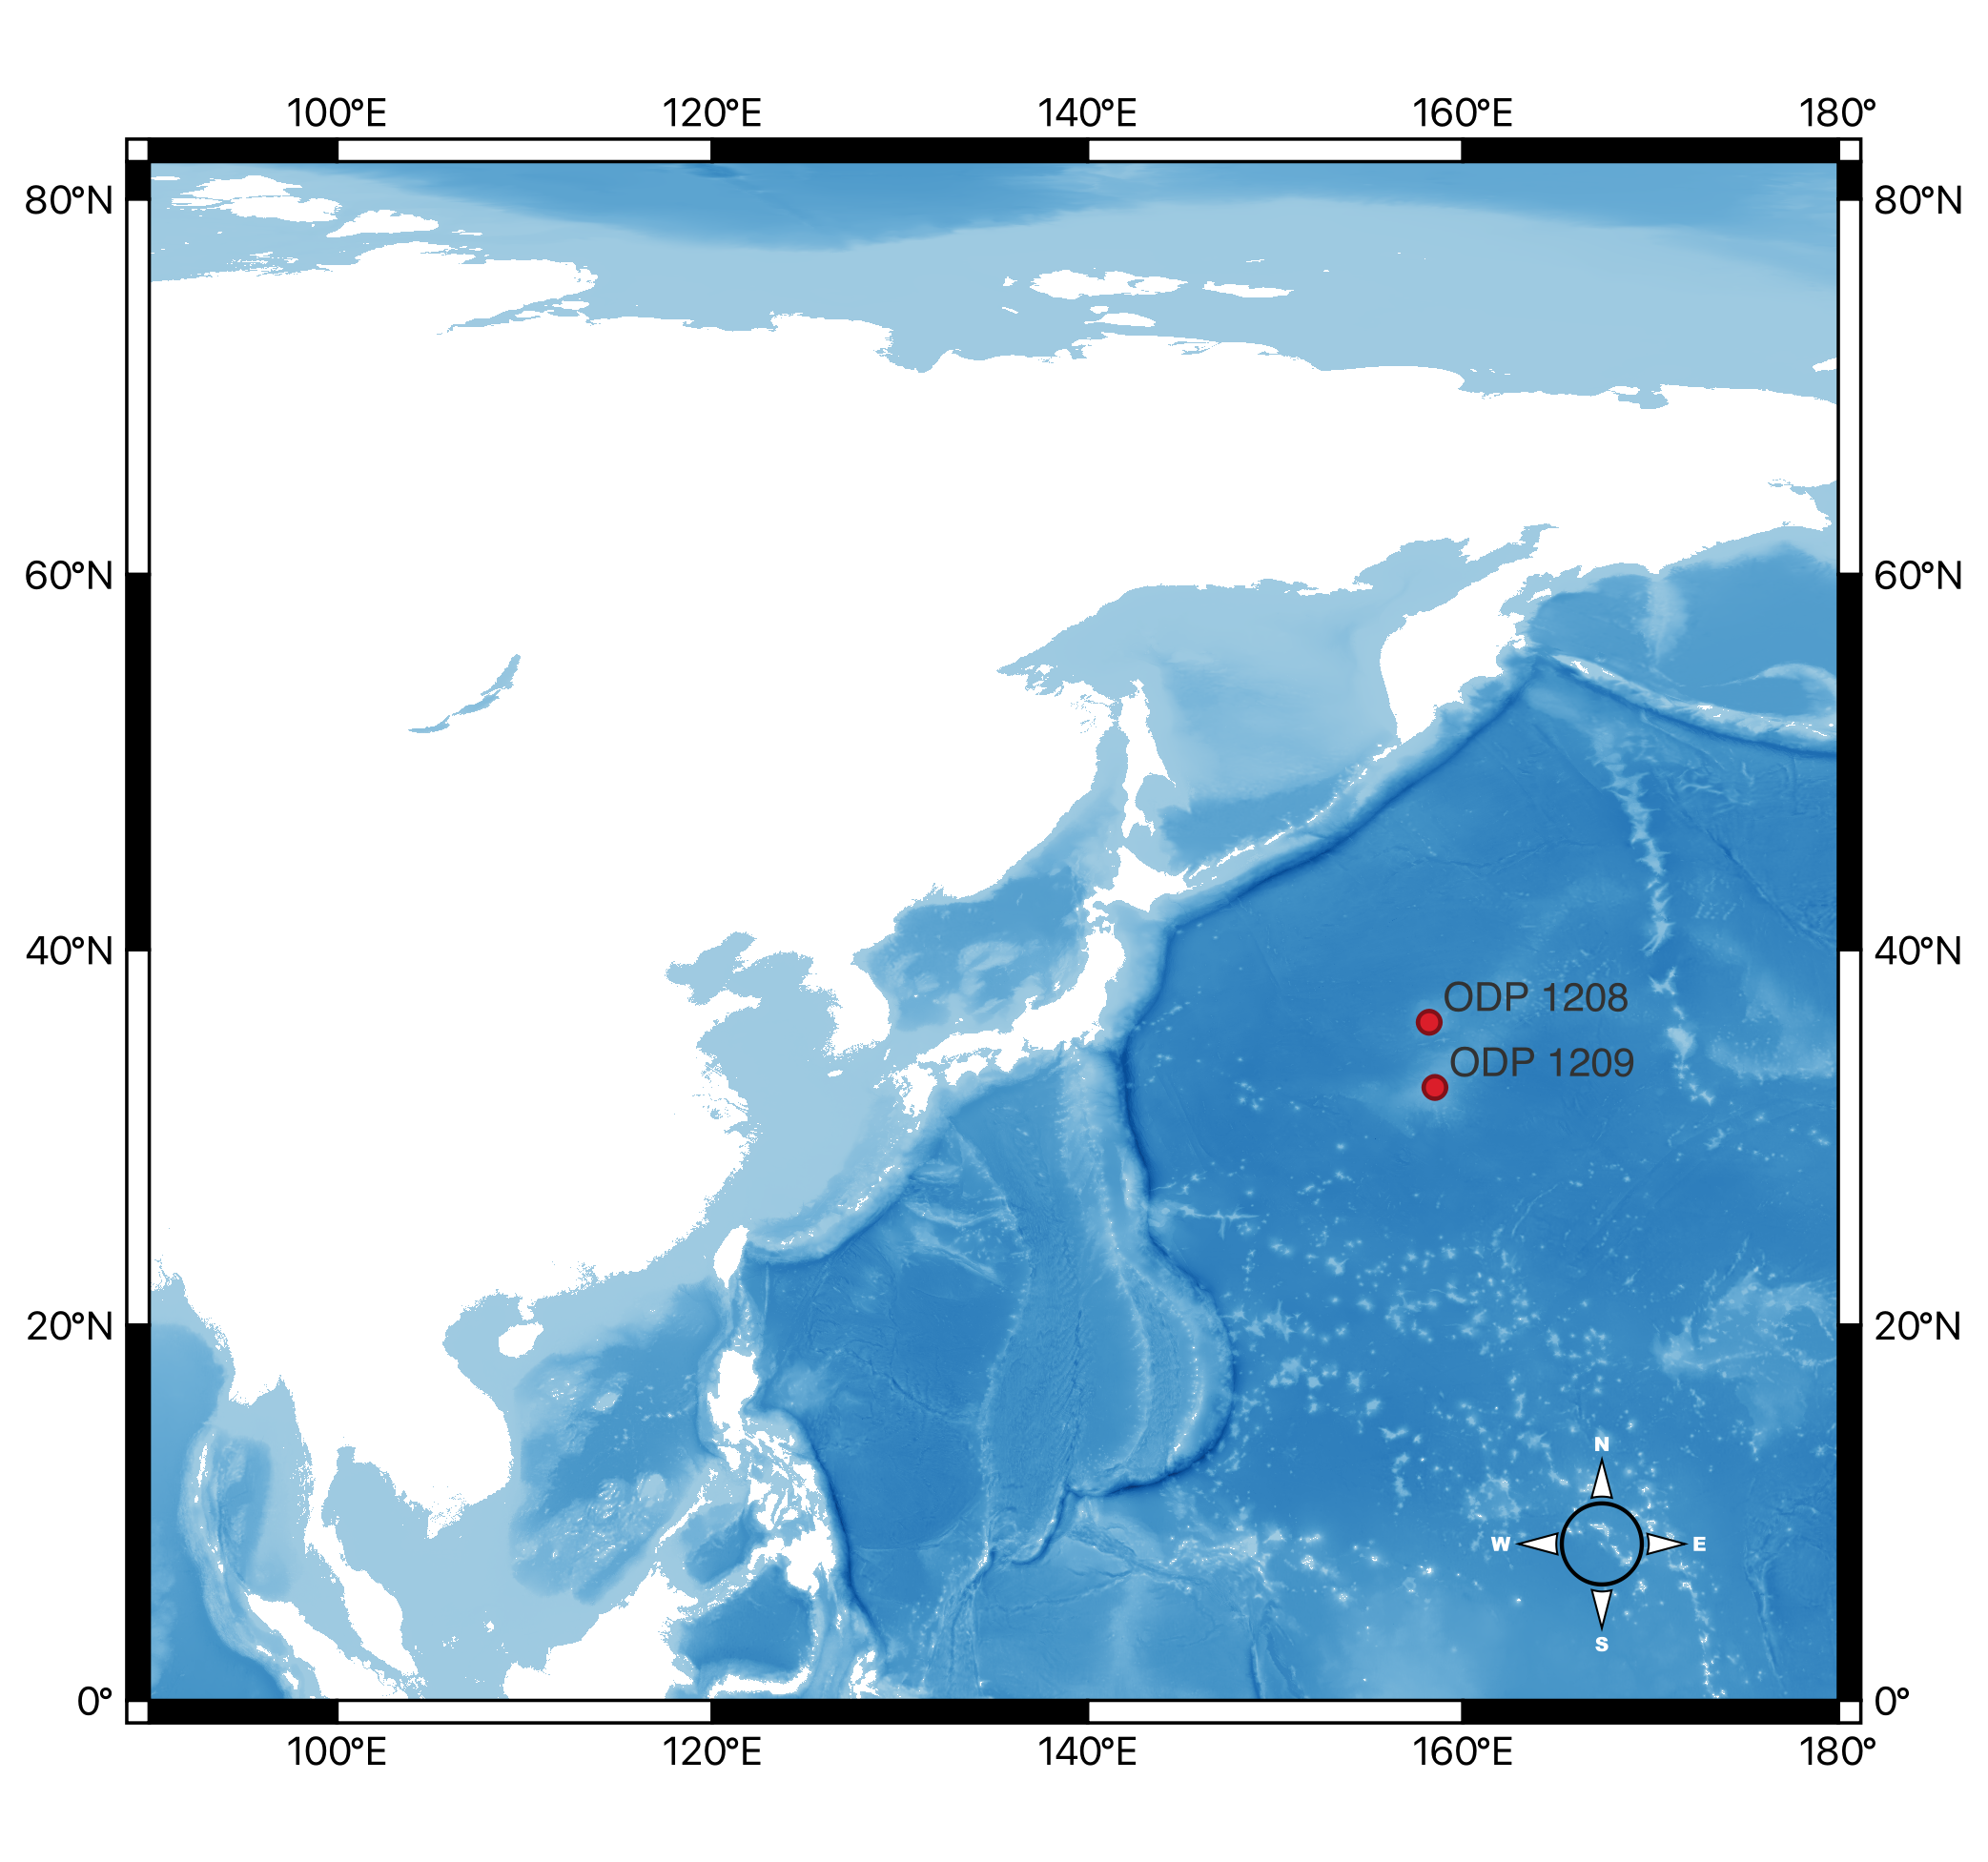
\includegraphics[width=0.7\textwidth]{NWPacific}
    \caption{Map of the North West Pacific Ocean showing the location of ODP Sites 1208 and 1209. From \citet{gebcobathymetriccompilationgroup2021GEBCO2021Grid2021}}
    \label{fig:NWPacific}
\end{figure}

The focus of this chapter of the project is to determine the physical characteristics of the intermediate and deep waters of the Pacific during the PMOC and after it has stopped. The project is looking at two sites in the North West Pacific Ocean, ODP Sites 1208 (3346 m depth) and 1209 (2387 m depth) \citep{bralowerLeg198Summary2002}. Their location (figure \ref{fig:NWPacific}) allows them to sample any deep waters that might form in the North Pacific which would then be carried southwards by deep western boundary currents \citep{fontelaNorthAtlanticWestern2020}. The lack of Pacific deep water formation means that both sites are bathed in the same poorly ventilated, nutrient-rich, southern-sourced water mass in the present day. In the Late Pliocene, active deep water formation would have resulted in a relatively fresh, cold, well-ventilated NPDW extending to approximately 3000 m depth (figure \ref{fig:DIC}) \citep{burlsActivePacificMeridional2017}. It is expected that site 1209 would be bathed in this fresher NPDW while the deeper site 1208 would only sample AABW from the Southern Ocean.

\newpage

\begin{figure}[h]
	\centering
	 \begin{subfigure}[b]{0.8\textwidth}
         	\centering
         	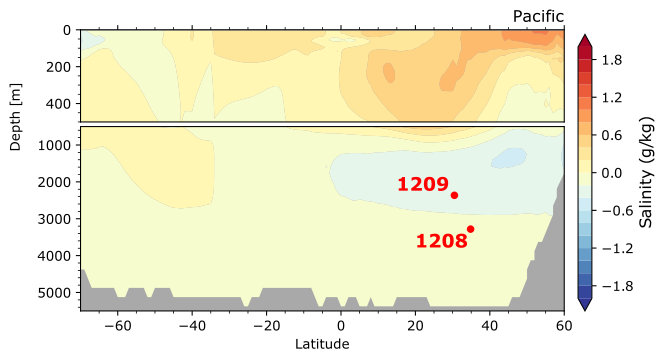
\includegraphics[width=\textwidth]{salinity}
         	\caption{Salinity}
     	\end{subfigure}
	\begin{subfigure}[b]{0.8\textwidth}
         	\centering
         	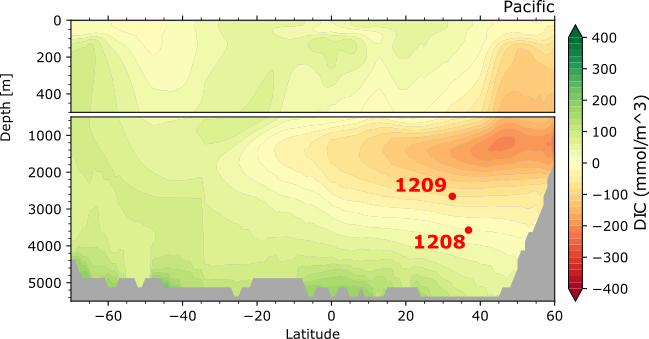
\includegraphics[width=\textwidth]{DIC}
         	\caption{DIC}
     	\end{subfigure}
   	 \caption{Model output showing salinity and dissolved inorganic carbon, DIC, in the Pacific Ocean in the Late Pliocene relative to the preindustrial. From \citet{fordSustainedMidPlioceneWarmth2022}}
    	\label{fig:DIC}
\end{figure}

\newpage

\subsubsection{Results and Discussion}

Oxygen isotope measurements were made on \emph{Cibicidoides wuellerstorfi} foraminifera from Site 1209 over the Late Pliocene and Early Pleistocene. There were compared to existing $\delta^{18}\text{O}$ records from the same time period from Site 1208 \citep{ventiPaleoproductivityNorthwesternPacific2017}. Positive $\delta^{18}\text{O}$ values are usually associated with colder or more saline, and thus denser, water masses. In the Late Pliocene, more positive $\delta^{18}\text{O}$ values are seen at Site 1209 compared to 1208, despite 1209 being the shallower site (figure \ref{fig:results_01}). This divergence in oxygen isotopes begins around 3.3 Ma and continues until the end fo the iNHG, around 2.5 Ma.

\begin{figure}[h]
    \centering
    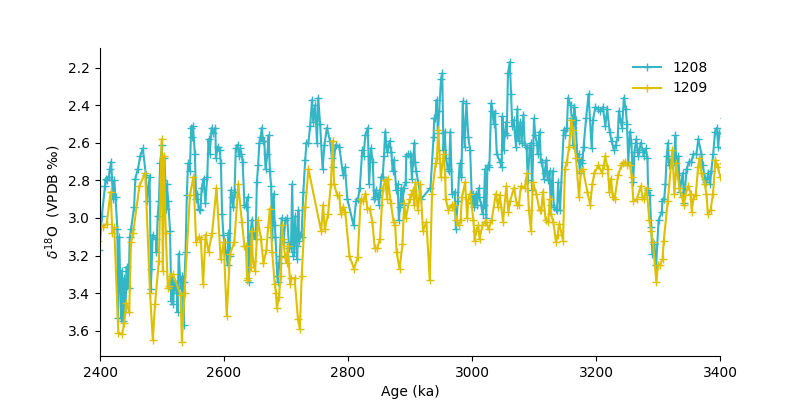
\includegraphics[width=0.9\textwidth]{Figure_1}
    \caption{Oxygen isotope measurements from \emph{Cibicidoides wuellerstorfi} from ODP Site 1208 \citep{ventiPaleoproductivityNorthwesternPacific2017} and 1209 (Ford, unpublished)}
    \label{fig:results_01}
\end{figure}

In the present day there is no major difference in oxygen isotope values between the two sites. The modern North Pacific is homogenous in oxygen isotopes, with the difference in intermediate and deep ocean $\delta^{18}\text{O}$ values being less than 0.465 \textperthousand (95\% confidence, figure \ref{fig:oceans_sup}). In the North and Southern Atlantic there is a greater heterogeneity between intermediate and deep waters, and the differences are generally less than 0.59\textperthousand and 0.72\textperthousand respectively (figure \ref{fig:oceans_sup}). This difference is driven by the deep water formation in the Atlantic which causes different water masses to overly one another. The difference in $\delta^{18}\text{O}$ regularly exceeds 0.6\textperthousand in the Late Pliocene, pointing to a different ocean structure in the Pliocene Pacific Ocean compared to the present.

The heavier oxygen isotopes at the shallower Site 1209 over Site 1208 requires a decoupling of $\delta^{18}$O values and salinity. The formation of AABW off the coast of Antarctica is driven in part by brine-rejection from the formation of sea ice, which increases the salinity of these surface waters without fractionating any oxygen isotopes, and would result in more saline, denser waters, without a correspondingly heavier $\delta^{18}\text{O}$ signal. A similar process occurs in the modern South Atlantic Ocean \citep{lynch-stieglitzMeridionalOverturningCirculation2006}. The greater $\delta^{18}$O values at 1209 could be explained by NPDW at this site being colder, but fresher, than the underlying AABW (figure \ref{fig:DIC}).

The $\delta^{18}\text{O}$ measurements from Sites 1208 and 1209 converge over the iNHG. This is likely due to the formation of a strong halocline in the North Pacific inhibiting NPDW formation. The oxygen isotope record converges more during glacials and less during interglacials indicating that the lower temperatures or greater ice volume of the Early Pleistocene may be responsible for suppressing NPDW formation.

Measurements of the Mg/Ca ratio were made of \emph{Uvigerina peregrina} foraminifera from Site 1209 over the iNHG. These results were compared to a similar record from Site 1208 \citep{woodardAntarcticRoleNorthern2014}, and both records were combined with $\delta^{18}\text{O}$ measurements in a bootstrap Monte Carlo model to solve for temperature and $\delta^{18}\text{O}_\text{sw}$ (figure \ref{fig:results_02}) \citep{thirumalaiConstrainingSeawater182016}. 

\begin{figure}[h]
    \centering
    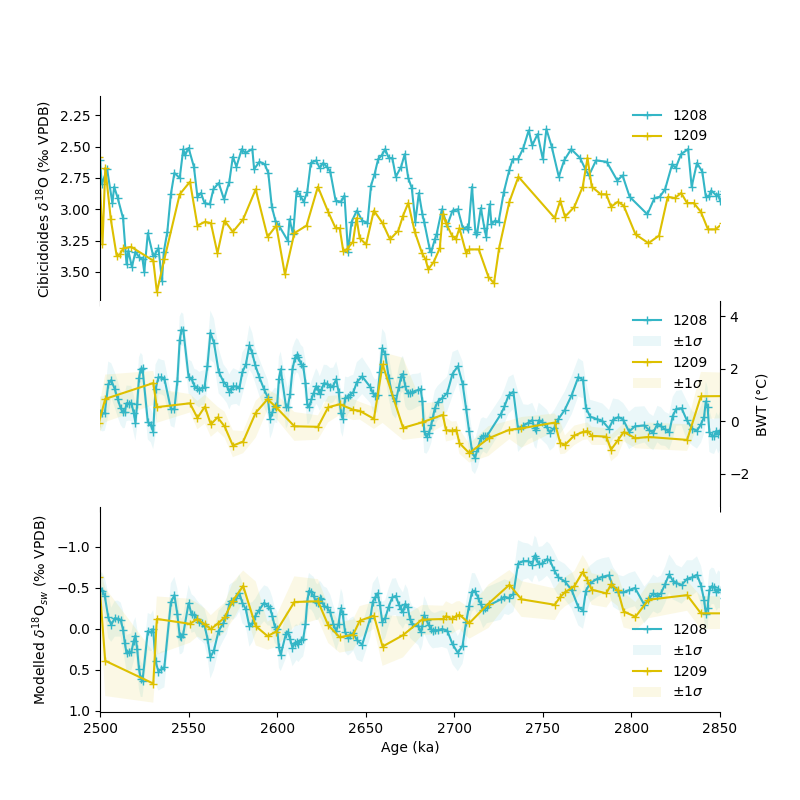
\includegraphics[width=0.9\textwidth]{Figure_2}
    \caption{Comparison of Mg/Ca derived BWT and $\delta^{18}\text{O}$ estimates from Sites 1208  \citep{woodardAntarcticRoleNorthern2014, ventiPaleoproductivityNorthwesternPacific2017} and 1209 (Ford, unpublished, and own work). Estimates of BWT and $\delta^{18}\text{O}_\text{sw}$ are generated using PSU Solver from \citet{thirumalaiConstrainingSeawater182016}}
    \label{fig:results_02}
\end{figure}

The BWT estimates from Site 1209 show colder temperatures than at 1208 for much of the iNHG, with converging driven by a slight warming at Site 1209 in the Early Pleistocene. The $\delta^{18}\text{O}_\text{sw}$ estimates, a proxy for salinity, show similar values for both sites within error. These results support the idea that Site 1209 is being bathed in fresher, colder, NPDW from an active PMOC in the Late Pliocene. The convergence in $\delta^{18}\text{O}$ over the iNHG is driven by a warming at Site 1209, likely reflecting an increased influence of AABW at the site as the PMOC is shut down. The convergence of BWT over the iNHG is more pronounced during glacials, with cooling at 1208 during glacial periods, contrasting with the gradually rising BWT at Site 1209. The glacial-interglacial variability in BWT at Site 1208 supports the idea of growing Pleistocene ice sheets playing a role in cooling the Southern Ocean over the iNHG. This could have led to an increase in deep water formation, encouraging the export of CDW and AABW from the Southern Ocean into the Pacific Basin. The gradual warming in BWT at 1209 suggests that if there is a shutdown in NPDW formation over the iNHG, it is not an instantaneous process centred on 2.73 Ma but occurs more gradually.

The record of BWT from 1209 is much less variable than that at 1208, particularly on glacial-interglacial timescales in the Early Pleistocene. This could reflect the increasing influence of ice sheet and sea ice expansion on the southern-sourced AABW \citep{hillModelledOceanChanges2017}, or could be the result of the low resolution of the 1209 Mg/Ca record having aliasing issues.

\begin{figure}[h]
    \centering
    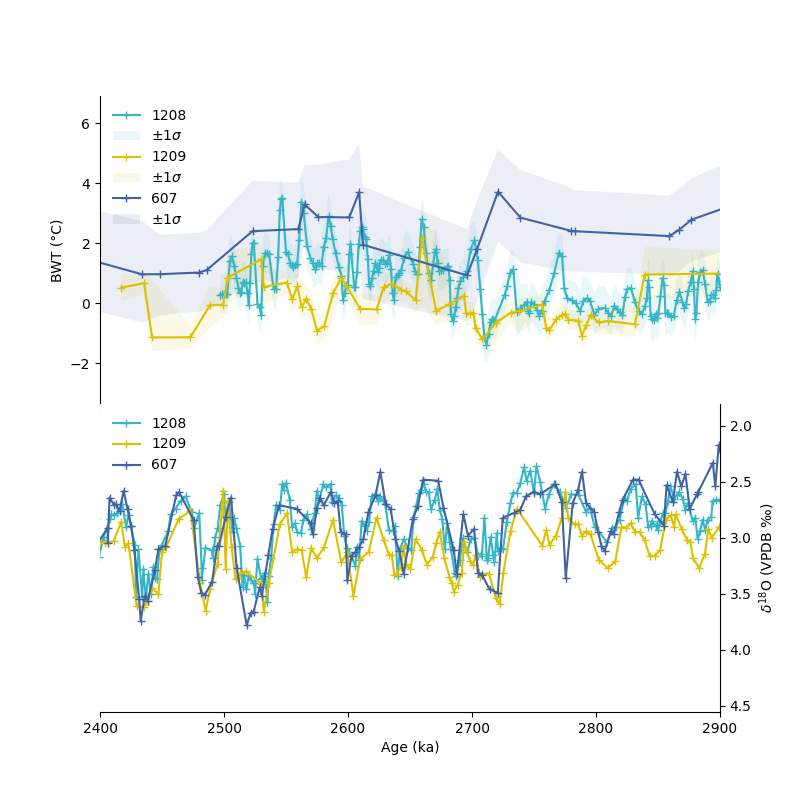
\includegraphics[width=0.9\textwidth]{Figure_3}
    \caption{Comparison of Mg/Ca derived BWT estimates for Sites 1209, 1208 \citep{woodardAntarcticRoleNorthern2014} and 607 \citep{sosdianDeepSeaTemperatureIce2009}}
    \label{fig:results_03}
\end{figure}

North Atlantic BWT records from Site 607 (figure \ref{fig:results_03}) also show a convergence with the BWT record at Site 1208, over a similar timescale to the convergence at Site 1209. DSDP Site 607 is located at 3426 m depth in the North Atlantic, and samples NADW exported from further North \citep{ruddimanInitialReportsDeep1987}. The BWT record at Site 607 shows a cooling over the iNHG, while the convergence at Site 1209 is driven by a warming in BWT. The opposite sign of temperature change at the two sites suggests that the convergence in North Pacific BWT is not driven by greater NADW import \citep{kwiekPacificOceanIntermediate1999}. 

The convergence of the deep water mass properties at all three sites (figure \ref{fig:results_03}) could indicate a common water mass bathing all three sites. This might be the result of stronger AABW and CDW export over the iNHG, due to an expansion in Antarctic sea ice, causing an increase homogeneity in Pacific and Atlantic water masses \citep{woodardAntarcticRoleNorthern2014}.

\subsubsection{Future Directions}

The next aim of this project is to undertake more measurements of the Mg/Ca ratios on foraminifera at Site 1209. More measurements in the Early Pleistocene will allow me to resolve whether the convergence in $\delta^{18}\text{O}$ and Mg/Ca values is influenced by glacial-interglacial cycles. A higher resolution record could show that BWT at Site 1208 and 1209 converges more during glacials and then diverges during interglacials, suggesting a strong role for ice growth in modulating the PMOC shutdown. The final convergence of the $\delta^{18}\text{O}$ records at 2.55 Ma, coincident with evidence for marine-terminating ice sheets in the Gulf of Alaska \citep{maslinProgressiveIntensificationNorthern1996}, suggests that ice sheet growth over the iNHG may have played a role in establishing a North Pacific halocline.

Alternatively, a higher resolution BWT record could show the waters at Site 1209 becoming gradually warmer with no apparent orbital forcing. This would imply that atmospheric moisture transport is more likely the main driver of halocline formation over the iNHG \citep{burlsActivePacificMeridional2017}. Increased meridional atmospheric moisture transport has been suggested as a factor in the initiation of the iNHG \citep{brierleyRelativeImportanceMeridional2010} and could explain the synchronous timings of the PMOC shutdown and the iNHG. 

Deep waters formed in the subpolar North Pacific would be more ventilated in the deep Pacific Ocean than those from the Southern Ocean (figure \ref{fig:DIC}). The NPDW formed from an active PMOC will have a lower dissolved inorganic carbon, DIC, content, and thus higher $\left[ \text{CO}_3^{2-}\right]$, than AABW. The difference in DIC can be seen in carbon isotopes \citep{fordSustainedMidPlioceneWarmth2022} and B/Ca measurements. The next steps are to undertake B/Ca measurements in \emph{Cibicidoides wuellerstorfi} from Site 1209 to compare to existing measurements from Site 1208 (Rosenthal, unpublished). The B/Ca measurements will give an estimate of how $\left[\text{CO}_3^{2-}\right]$ values changed over the iNHG. 

It is expected that the $\left[ \text{CO}_3^{2-}\right]$ values would be higher at Site 1209 than 1208 during the Pliocene, reflecting the DIC-poor, well-ventilated NPDW bathing Site 1209 (figure \ref{fig:DIC}). A similar structure is seen in the modern North Atlantic, where the well-ventilated NADW has a higher $\left[ \text{CO}_3^{2-}\right]$ content than the underlying poorly ventilated AABW \citep{chalkDynamicStorageGlacial2019}. 

The results could show similar $\left[ \text{CO}_3^{2-}\right]$ values at both Site 1208 and 1209. This is similar to the situation in the modern Pacific Ocean where there is little heterogeneity in DIC content. This could therefore reflect the absence of a PMOC in the Late Pliocene. Equally, it could show that NPDW formation occurs in a nutrient-rich, upwelling environment, in contrast to NADW which forms from nutrient-limited surface waters \citep{skinnerAtlanticOceanVentilation2020}. The idea of a nutrient-rich NPDW is supported by high opal accumulation rates in the Late Pliocene subpolar North Pacific \citep{haugNorthPacificSeasonality2005,swannSalinityChangesNorth2010}. If this were the case, it would imply that CO$_2$ storage of the deep Pacific was not hugely different in the Pliocene relative to the present. The Pacific Ocean is a major store of carbon \citep{chengImprovedEstimatesOcean2017}, and so this would suggest that the higher CO$_2$ levels of the Late Pliocene were not driven by Pacific Ocean changes \citep{bartoliAtmosphericCO2Decline2011}. 

The B/Ca measurements from Site 1209 may also indicate lower $\left[ \text{CO}_3^{2-}\right]$ values than at 1208. If this were the case, it would suggest that the formation of deep waters in the Southern Ocean is likely different to today, with greater degassing and ventilation causing higher $\left[ \text{CO}_3^{2-}\right]$ values in the Late Pliocene AABW.

\subsection{Changes in AMOC Strength}

The changes in AMOC strength over the iNHG are poorly understood, with evidence pointing to a stronger, weaker and unchanged overturning circulation during the iNHG \citep{raymoResponseDeepOcean1992, hayashiLatestPlioceneNorthern2020, langIncursionsSouthernsourcedWater2016}. The AMOC is a key driver of ocean circulation \citep{talleyChapterAtlanticOcean2011} and has major impacts on ocean structure in the Pacific and Atlantic basins.

The strength of the AMOC overturning is usually derived from proxies for the spatial extent of NADW, with a greater extent of NADW implying a stronger AMOC. However, the extent of NADW is dependent on AMOC strength but also the export of water masses in the Southern Ocean. There are many studies from the North \citep{hayashiLatestPlioceneNorthern2020, langIncursionsSouthernsourcedWater2016} and South \citep{hodellHighResolutionStableIsotopic1992,raymoResponseDeepOcean1992} Atlantic over the iNHG but few from the mid-Atlantic where the extent of NADW could be most clearly seen. This project will reconstruct the BWT, $\left[ \text{CO}_3^{2-}\right]$ and $\varepsilon_\text{Nd}$ in the Central Atlantic to characterise and understand the spatial extent of northern and southern-sourced deep waters. This will allow us to better constrain the spatial extent of the NADW in the mid-Atlantic over the iNHG and infer how AMOC strength may have changed.

\begin{figure}[h]
    \centering
    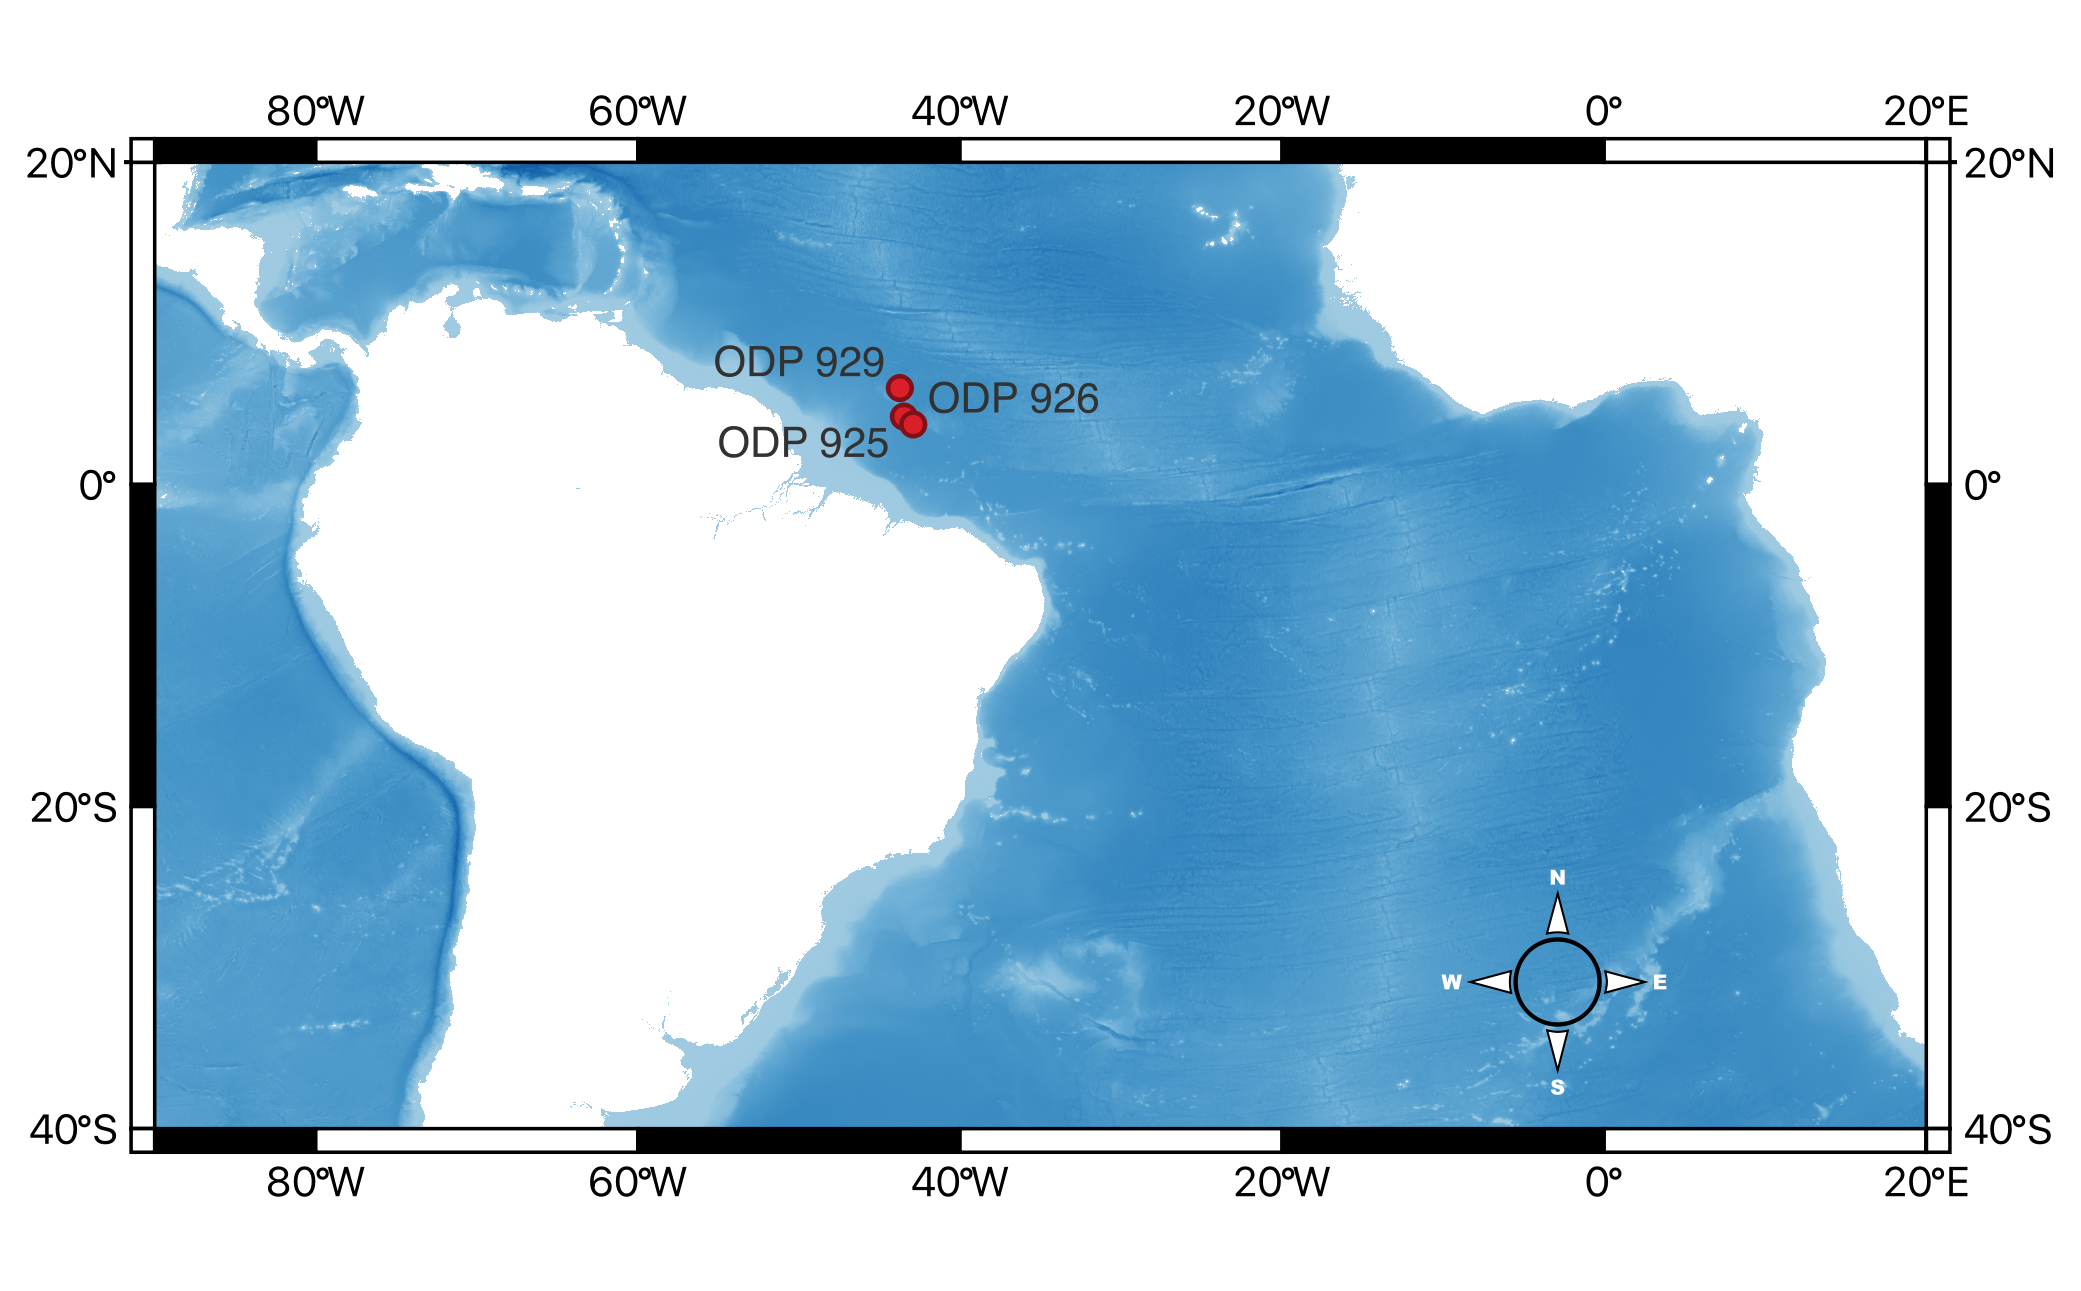
\includegraphics[width=0.7\textwidth]{CAtlantic}
    \caption{Map of the Central Ocean showing the location of ODP Sites 925, 926 and 929. From \citet{gebcobathymetriccompilationgroup2021GEBCO2021Grid2021}}
    \label{fig:CAtlantic}
\end{figure}

This study will look at ODP Sites 925, 296 and 929 in the Central Atlantic (figure \ref{fig:CAtlantic}). These sites are located on the Ceara Rise, off the coast of Brazil, at depths of 3042 m, 3609 m, and 4369 m depth respectively \citep{curryProceedingsOceanDrilling1995}. The modern day boundary between AABW and NADW in the Central Atlantic sits around 4000 m depth \citep{curryProceedingsOceanDrilling1995}, and so these sites are well suited to determining how this boundary has changed over time in response to circulation strength.

The first aim of this project will be to generate an Mg/Ca record for the three sites. This record will focus on the Late Pliocene interglacial KM5c (c. 3.205 Ma) and the Early Pleistocene glacials and interglacial MIS 100 and 99 (2.50 - 2.52 Ma) (figure \ref{fig:results_04}). These periods, before and after the iNHG, will allow for a good reconstruction of the changes that occurred over this transition. The results from interglacial KM5c can be compared with the results from the PlioVAR data synthesis project \citep{mcclymontLessonsHighCO2World2020}, and the PlioMIP model intercomparison project \citep{haywoodPlioceneModelIntercomparison2020}, which both focus on this interval. This interglacial is thought to be representative of a ``normal'' Late Pliocene climate state. In the Early Pleistocene there are several records from the North Atlantic which cover MIS 100 and 99 \citep{ohnoMillennialScaleInteractionIce2016, groeneveldGlacialInducedClosure2014} allowing for detailed comparison.

\begin{figure}[h]
    \centering
    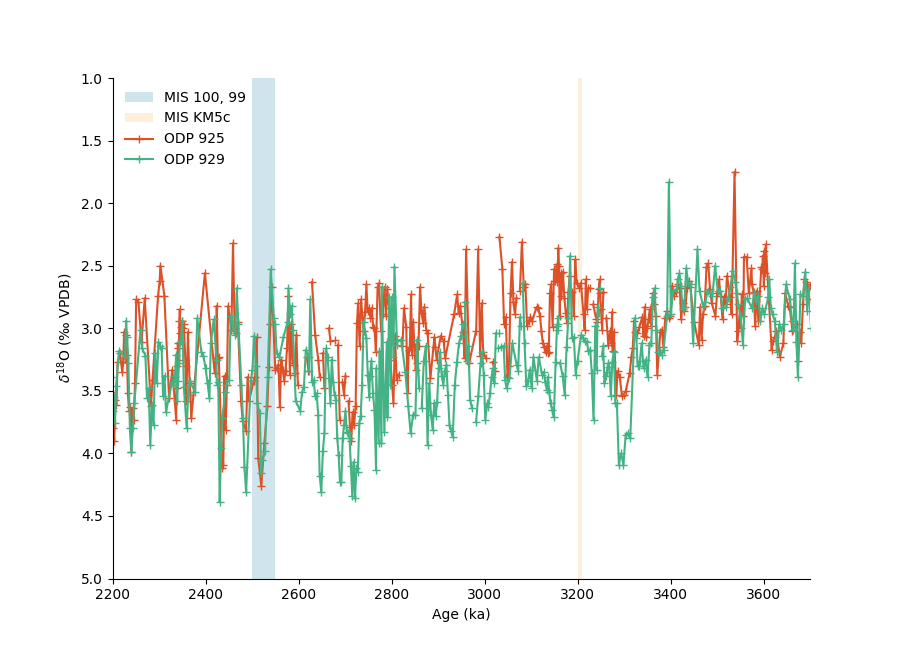
\includegraphics[width=0.9\textwidth]{Figure_4}
    \caption{ $\delta^{18}\text{O}$ records from the intermediate (Site 925) and deep (Site 929) Central Atlantic Ocean over the iNHG. Shaded regions show MIS KM5c (3.21 - 3.22 Ma) and MIS 100, 99 (2.50 - 2.52 Ma). Data from \citet{wilkensRevisitingCearaRise2017}}
    \label{fig:results_04}
\end{figure}

The Mg/Ca record from these sites will be used to determine how BWT changed across a depth-transect of the Central Atlantic Ocean over the iNHG. These results will be compared to existing $\delta^{18}\text{O}$ measurements from the sites (figure \ref{fig:results_04}) \citep{wilkensRevisitingCearaRise2017} to estimate how $\delta^{18}\text{O}_\text{sw}$ may have changed. The existing records show a convergence in $\delta^{18}\text{O}$ between Sites 929 and 925 from the Late Pliocene to the Early Pleistocene (figure \ref{fig:results_04}). The Mg/Ca results from before and after the iNHG should help to deconvolve why this convergence occurred.

The BWT record at Sites 925 and 926 could show a cooling, converging with the expected colder temperatures at Site 929. This would match what is seen at Site 607 over the iNHG \citep{sosdianDeepSeaTemperatureIce2009, woodardAntarcticRoleNorthern2014} with a cooling in NADW temperatures to match the BWT from southern-sourced waters. This result would imply that there is a greater ``Antarctic'' influence on waters in the deep Atlantic, either due to an increase in CDW export or a decrease in AMOC strength over the iNHG.

Alternatively, the Mg/Ca measurements may show very little change in BWT over the iNHG, which would indicate that the convergence in $\delta^{18}\text{O}$ between Sites 925 and 929 (figure \ref{fig:results_04}) is driven by salinity changes rather than temperature changes. This would be a different pattern to what is seen in the North Pacific but could be driven by an increase in salinity in the North Atlantic. An increase in salinity in the North Atlantic coincident with a freshening in the North Pacific suppressing NPDW formation would imply a strong salt transport from the Pacific to the Atlantic over the iNHG \citep{woodardAntarcticRoleNorthern2014}. 

An issue to consider is whether the convergence in $\delta^{18}\text{O}$ between Sites 925 and 929 over the iNHG is driven by a change in water mass properties or due to all the sites being bathed in the same water mass. The second part of the project will undertake B/Ca measurements on benthic foraminifera from the three sites, 925, 926 and 929, over the same intervals before and after the iNHG. 

AABW forms in a nutrient-rich upwelling zone in the Southern Ocean and so will have a lower $\left[ \text{CO}_3^{2-}\right]$ content than NADW which forms in nutrient-limited subpolar North Atlantic. The B/Ca measurements can be used as a water mass tracer to infer which water mass is bathing which site. 

A decrease in $\left[ \text{CO}_3^{2-}\right]$ content over the iNHG at the shallower Site 925 could suggest that the site is being bathed in southern-sourced deep waters \citep{langIncursionsSouthernsourcedWater2016}. This would point to a weaker AMOC or a stronger Southern Ocean deep water export over the iNHG.  Alternatively, lower $\left[ \text{CO}_3^{2-}\right]$ values could imply that there is a change in the ventilation structure of the deep North Atlantic. This could come about through an increased influence of poorly-ventilated, $\left[ \text{CO}_3^{2-}\right]$-poor Nordic Seas waters into the NADW, as has been suggested for the Last Glacial \citep{larkinActiveNordicSeas2022}. However, other indicators for the North Atlantic do not suggest that there was a major change in ventilation patterns over the iNHG \citep{drautClimateStabilityPliocene2003}.

Alternatively, if there was little change in the $\left[ \text{CO}_3^{2-}\right]$ values measured at the three sites over the iNHG, this would imply that the structure of the deep Central Atlantic Ocean did not change over the iNHG. This would mean that the convergence in $\delta^{18}\text{O}$ values is driven by a change in water mass properties, either in the North Atlantic or the Southern Ocean.

A change in $\left[ \text{CO}_3^{2-}\right]$ values at a site could be the result of a change in nutrient utilisation or ventilation of water masses, or it could be the result of a change in the water mass bathing that site. The project will follow up with $\varepsilon_\text{Nd}$ measurements at the three sites over the study intervals to determine the provenance of the particular water masses at each site. It is expected that, similar to today, NADW sourced from surface waters in the North Atlantic will have much more negative $\varepsilon_\text{Nd}$ values than waters sourced from the Southern Ocean \citep{vandeflierdtNeodymiumOceansGlobal2016}. 

The end-member compositions of either NADW or AABW may be different in the Late Pliocene or Early Pleistocene compared to the present. Comparison with other $\varepsilon_\text{Nd}$ records from the Pliocene North Atlantic \citep{langIncursionsSouthernsourcedWater2016} will help to constrain the $\varepsilon_\text{Nd}$ signal of NADW which will allow for better reconstructions of water mass provenance.

\subsection{Effects on Volcanism}

The final chapter of this project will look at how volcanism may have changed in response to the iNHG. Volcanism is a major driver of past climatic change \citep{mckenzieContinentalArcVolcanism2016} and so understanding the drivers of volcanism is key to understanding past climates. 

The aim of this chapter of the project is to construct a record of volcanism on Iceland for the Late Pliocene and Early Pleistocene from tephra in marine sediments cores, and to determine if there is a significant change in the rate of volcanism over the iNHG on Iceland. The most effective method of inferring changes in the strength of volcanism over the iNHG is to look at marine tephra records from the Late Pliocene. Tephra records provide the most accessible way of inferring past rates of volcanism and marine cores are the only locations where these sediments are preserved over this time period \citep{cassidyConstructionVolcanicRecords2014}. 

\begin{figure}[h]
    \centering
    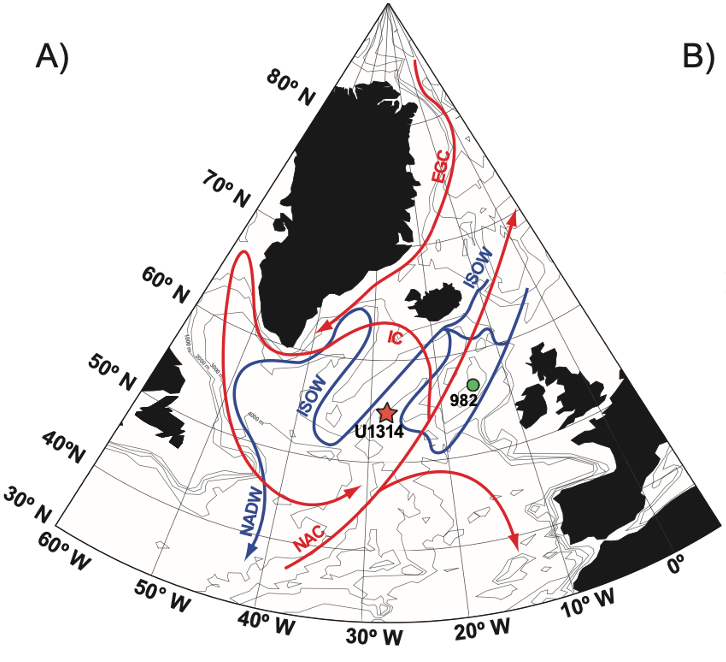
\includegraphics[width=0.9\textwidth]{tephra_map}
    \caption{The location of U1314 in the Northeast Atlantic Ocean showing also the ODP Site 982 and the location of major deep (blue) and surface (red) ocean currents. From \citet{hernandez-almeidaSubsurfaceNorthAtlantic2014}}
    \label{fig:tephra_map}
\end{figure}

The first part of this chapter will look at tephra layers at IODP Site U1314 in the North East Atlantic Ocean (figure \ref{fig:tephra_map}). This site is located directly south of Iceland, on the Gardar Drift, and so will be able to sample tephra ejected from Icelandic volcanism. There is reasonable tephra preservation at the site for the last glacial \citep{abbottTracingMarineCryptotephras2018}, though typically tephra from Iceland volcanism is carried to the southeast \citep{daviesWidespreadDispersalIcelandic2010}. Initial studies have noted the presence of tephra in Pliocene sections of U1314 \citep{channellMagneticRecordDeglaciation2016}. If there are sufficiently high tephra counts at the site, the relative change in tephra deposition before and after the iNHG could be used to infer the rate of volcanism over the transition.

There exists a magnetostratigraphic age model for the Site U1314 for the Early Pleistocene \citep{ohnoDetailedPaleomagneticRecord2012}, but not for the Late Pliocene. Therefore, this project will measure the $\delta^{18}\text{O}$ of benthic foraminifera to tie these measurements to the global ProbStack oxygen isotope record \citep{ahnProbabilisticPliocenePleistocene2017}. From these tie points, the aim is to make an age model for the Late Pliocene at Site U1314.

If there is a reliable tephra record at U1314, a tephra record will be generated for ODP Site 982 over the same period (figure \ref{fig:tephra_map}). There already exists an age model for Site 982 covering the iNHG \citep{khelifiTechnicalNoteLate2012}. A greater spatial extent of tephra records over the iNHG will add strength to any conclusions about the rate of volcanism over the iNHG. These two records are from far enough apart in the Northeast Atlantic Ocean that local factors, such as dissolution or ice-rafting of tephra, are unlikely to have a major impact on conclusions drawn from the two records.

If there is a decrease in tephra layers then this will likely be the result of increased ice loading on Iceland causing an increase in subsurface pressure. This increase in pressure will decrease the degree of magmatic melting which is linked to volcanism \citep{schmidtEffectsPresentdayDeglaciation2013,maclennanLinkVolcanismDeglaciation2002}. 

If there is an increase in tephra layers over the iNHG, this would suggest that the rate of volcanism increased on Iceland over the iNHG. This may be due to fracturing of the crust with the advance and retreat of ice sheets in the Early Pleistocene allowing more pathways for magma to rise to the surface \citep{jellinekDidMeltingGlaciers2004}. 

There may be insufficient tephra at Site U1314 to draw any conclusions about the changes in volcanism over the iNHG. In this case, the $\delta^{18}\text{O}$ record from Site U1314 will be augmented with Mg/Ca measurements on benthic foraminifera from Site U1314 from before and after the iNHG. The coupled BWT and $\delta^{18}\text{O}_\text{sw}$ estimates will allow for a better understanding of how NADW changed over the iNHG. Site U1314 is bathed in Iceland-Scotland Overflow Water (ISOW), a major component of NADW that is formed from cold surface waters in the Arctic and Nordic Seas \citep{xuVariabilityIcelandScotland2018}. If this record shows a cooling in BWT over the iNHG, akin to what is seen at Site 607 \citep{sosdianDeepSeaTemperatureIce2009}, then this would suggest that the convergence in deep water properties over the iNHG between the Atlantic and Pacific Oceans is driven by a cooling in NADW \citep{woodardAntarcticRoleNorthern2014} rather than an increased influence of AABW, which is unlikely to influence deep waters this far north. 







